\section{Introduction}
\label{sec:introduction}

		\Ac{vbl} consists of retrieving the pose (position + orientation) of a visual query material within a known space representation. For instance, recovering the pose of a camera that took a given photography according to a set of geo-localized images or a 3D model is a simple illustration of such a localization system. \ac{vbl} has been an increasingly dynamic research subject in the last decade. This recent gain of interest is due to the provision of large geo-localized images database, the multiplication of embedded visual acquisition system (\textit{e.g}. camera on smart-phone) and the limitation of usual localization system in urban environment (\textit{e.g.} GPS signal failure in cluttered environment). Aforementioned localization problem is involved in several present-day practical applications, such as GPS-like localization system, indoor or outdoor navigation, 3D reconstruction, models and databases update, consumer photography---``Where did I take these photos?''---and augmented reality. Visual-based localization is also used in robotics to solve SLAM loop-closure problem or «kidnapped robot» scenario.
		
		There is no standardized designation for \ac{vbl}, methods name vary from one paper to another. In this survey, we include in Visual-based Localization methods categorized as: Image-based localization~\citep{Azzi2016}, Visual localization \cite{Torii2011}, Structure-based localization~\citep{Sattler2015}, Visual geo-localization~\citep{Zamir2016,Brejcha2017}, Camera Relocalisation~\citep{Shotton2013}, Image-based pose estimation \citep{Heisterklaus2014}, and all the possible rearrangement of these terms.

	\begin{figure}[!ht]
	\centering

	\subfigure[][Indirect method]{\label{fig:indirect}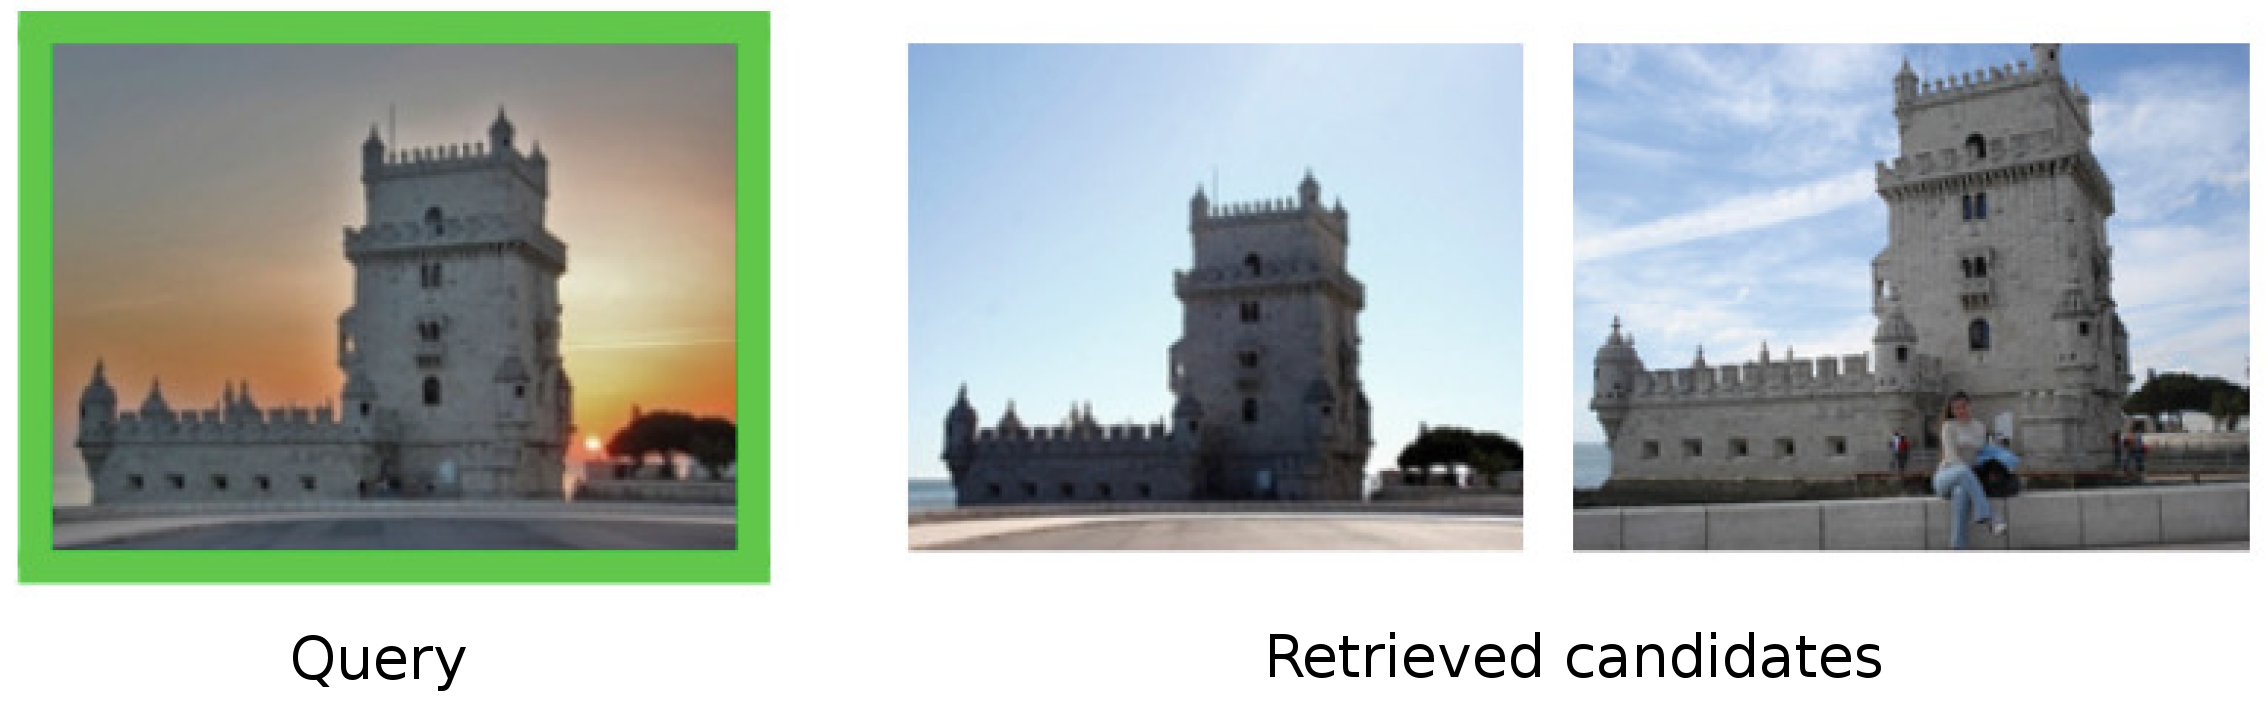
\includegraphics[width=0.5\linewidth]{intro/indirect.png}}
	\subfigure[][Direct method]{\label{fig:direct}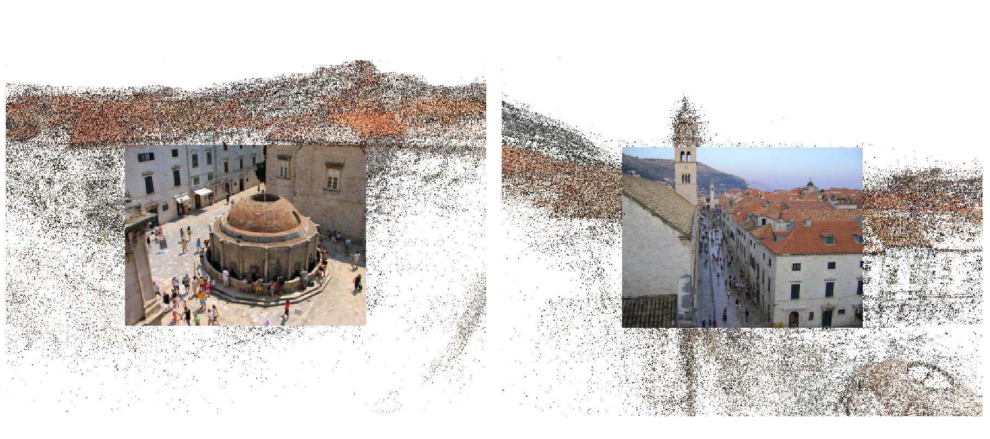
\includegraphics[width=0.48\linewidth]{intro/direct2.png}}
	\caption[Examples of Visual Based Localization systems]{\textbf{Examples of Visual Based Localization systems.} \ref{fig:indirect} -- indirect method from \citep{Arandjelovic2017}: according to an input query (left images), indirect methods recover a set of similar data (right images). \ref{fig:direct} -- direct method from~\citep{Feng2016a}: direct methods recover the exact pose of the input query (the two figures represents superposed images according to a reference 3D model). \label{fig:vbl_overview}}
\end{figure}

	
	\subsection{Topics addressed}
		Along the whole survey, we will focus on urban \ac{vbl} as it represents the most studied end-user application in literature. This can be explained by the fact that most of the related applications take place in non-rural environment. As an illustration, \ac{vbl} as GPS pedestrian localization system should be used when buildings (so inside a city) disrupt the satellite signal. Most of the augmented reality applications are also designed for indoor or urbanized environment. Similar reasoning can be employed with robotic applications. Nowadays principal concerns about robots are related to human assistance or supervision and autonomous vehicles. Those services occur in indoor and outdoor man-made areas, therefore the robot localization should be studied for these sites. The other aspect that invites researchers to focus on urban environment is that large datasets are mainly describing cities or road networks, because they are the most reachable places. With the exception of airborne and satellite imageries, that are abundant all over the globe but these data restrict the range of possible uses.
				
		As well as \ac{vbl} presents a heterogeneity about its end-user applications, methods and data involved in the process of localizing an image are various. These methods are divided into two categories: \textbf{indirect methods}~\citep{Arandjelovic2012,Radenovic2016} (see figure~\ref{fig:indirect}) that cast the localization task as an image retrieval problem and provide a coarse pose information about the query location and \textbf{direct methods}~\citep{Kendall2015,Sattler2016a} (see figure~\ref{fig:direct}) that directly regress the 6 \ac{dof} pose of the visual acquisition system. Indirect methods used in \ac{vbl} slightly differ from classical vision object-retrieval algorithm~\citep{Sivic2003} on two points: the images in the query and the database represent scenes rather than objects (\textit{e.g.} street view panorama, buildings images, indoor scenes) and the performance of such system is evaluated according to the precision rate rather than the recall rate (i.e. a perfect \ac{vbl} system should recover in its top ranked candidates documents that display the exact location of the query). Unlike indirect methods, direct methods aim to recover instantly the pose of the query data. Where \ac{sfm} or SLAM techniques provide a \textit{relative pose} of a sequence of data, \ac{vbl} tackles the problem of retrieving the \textit{absolute pose} of a query data according to a known representation. Nevertheless, this representation could have been built thanks to \ac{sfm} or SLAM mapping module.
Figure~\ref{fig:vbl_overview} presents representatives of the two different methods studied in this survey.
			
		When designing a \ac{vbl} system, the type of method is not the only parameter to consider. As pointed out in~\citep{Lowry2016}, robustness to environment appearance changes over time is a main concern. Data involved in the process of localization also define specifications of the system, like area covered by the \ac{vbl} method or precision of the regressed pose.  Data types are various in \ac{vbl}: visual data, geometric information (provided by RGB-D camera, LIDAR, etc.) and semantic clues. Combination of different data in \ac{vbl} aims to overcome limitation of images-only based method.
		
	\subsection{Related works} 
    	\ac{vbl} is a well studied topics, and many contributions propose overview of this domain. The closest survey to ours is the paper of \citet{Brejcha2017}. It presents many works on \ac{vbl} and classify them depending on the environment for which the particular method was developed. Conversely, we focus our study on systems built for city-scale localization as it concerns the most \ac{vbl} applications. Moreover, we propose a comprehensive description of the two types of methods used in \ac{vbl}, and highlight the benefits of the use of heterogeneous data in the context of localization in challenging scenarios. \citet{Zamir2016} gather recent articles to draw a large panorama of \ac{vbl}, corroborating the growing importance of this domain in current research. This assumption is comforted regarding the many tutorials (\href{https://sites.google.com/site/lsvpr2014/}{CVPR2014}, \href{https://roboticvision.atlassian.net/wiki/display/PUB/CVPR+2015+Workshop+on+Visual+Place+Recognition+in+Changing+Environments}{CVPR2015} and \href{https://sites.google.com/view/lsvpr2017/home}{CVPR2017}) and workshop (\href{https://roboticvision.atlassian.net/wiki/display/PUB/CVPR+2015+Workshop+on+Visual+Place+Recognition+in+Changing+Environments}{CVPR2015}) about the Visual Localization problem in high impact international conferences.
    	
		Visual Place Recognition is a roboticist problem, defined in the general sense in~\citep{Lowry2016} as the visual ability of a human, an animal or a robot to recognize an already visited place. It is a main concern for navigation, especially when we consider topological mapping~\citep{Garcia-Fidalgo2015}. Despite the fact that Visual Place Recognition shares huge similarity with the issues addressed in this survey, the two problems differ on three major points. On the one hand, visual-based localization and visual place recognition purposes differ; where Place Recognition decides if a given place have already been seen, \ac{vbl} produces a pose of the visual acquisition system. This explains the difference in their respective pipeline. Visual place recognition is composed of three main components (the data processing module, the mapping module and the belief generation modules) while visual-based localization does not consider the mapping module. On the other hand, the study presented here aims to consider \ac{vbl} in a more general context. Communities and applications of the reviewed methods belong to the Computer Vision community~\citep{Sattler2011}, as well as the Robotic~\citep{Garcia-Fidalgo2015} and the Photogrammetric communities~\citep{Wan2016}. Finally, in this survey, we consider \textit{heterogeneous} visual data without restriction, including: raw colour and grey-scale images, depth images, point cloud and 3D models, as well as semantic information extracted from aforementioned data. 
	
		However, we advise reader to refer to the recent surveys related to Visual Place Recognition~\citep{Lowry2016,Garcia-Fidalgo2015,Kostavelis2015} in order to capture a global panorama of existing approaches involved in localization process with visual data.		

		\bigskip
		The rest of the paper is organized in two parts: on the one hand we study two different methods, introducing in Section~\ref{sec:image_representation} several data representations used in \ac{vbl} followed by description of indirect (Section~\ref{sec:matching}) and direct (Section~\ref{sec:fine_pose_estimation}) systems; the second part focus on data involved in \ac{vbl}, with in Section~\ref{sec:changing_environment} an analysis of the problem of challenging association across data variability and in Section~\ref{sec:application} an overview of the different type of database and query used in \ac{vbl}; finally, in Section~\ref{sec:comparison}, trends and representative methods are discussed and Section~\ref{sec:conclusion} concludes this work.